\section{Phát hiện và giải thích bất thường theo ngữ cảnh dựa trên phân vị}
\label{sec:qcad}

Chúng tôi trình bày một ví dụ về cách tiếp cận chung để phát hiện sự bất thường theo ngữ cảnh được trình bày trong Phần~\ref{subsec:framework} dựa trên các khu rừng hồi quy phân vị.

Ý tưởng chính của phương pháp của chúng tôi là ước tính độ lệch của các giá trị hành vi của một đối tượng trong một bối cảnh nhất định bằng cách sử dụng định lượng độ không đảm bảo xung quanh các dự đoán, trong đó các dự đoán được giả định là nắm bắt được hành vi 'bình thường'. Sau đó, độ không chắc chắn cao hơn hàm ý độ lệch cao hơn trong bối cảnh và do đó mức độ bất thường cao hơn. Để đạt được mục đích này, một số cách tiếp cận có thể được khám phá. Ví dụ: người ta có thể sử dụng các mô hình hồi quy đa mục tiêu---chẳng hạn như Rừng ngẫu nhiên đa biến \citep{segal2011multivariate}---trên tất cả các đặc trưng hành vi hoặc mô hình hồi quy một mục tiêu---chẳng hạn như Rừng ngẫu nhiên \citep{breiman2001random}---trên các đặc trưng hành vi riêng lẻ, sau đó là tổng hợp và suy luận tuân thủ \citep{lei2018distribution}. Thay vào đó, trong bài viết này, chúng tôi chọn sử dụng Rừng hồi quy phân vị \citep{meinshausen2006quantile}, một mô hình hồi quy một mục tiêu, vì nó (tương đối) đơn giản, mang lại lợi thế về khả năng diễn giải và trực tiếp cung cấp định lượng không chắc chắn. Cụ thể hơn, chúng tôi rút ra các khoảng thời gian cho các đặc trưng hành vi từ các khu rừng hồi quy phân vị cơ bản dưới dạng định lượng không chắc chắn cố hữu xung quanh các dự đoán, dẫn đến các biện pháp thống kê hợp lý và có thể giải thích được về mức độ bất thường.

Trong giai đoạn đầu tiên, chúng tôi tạo các nhóm tham chiếu bằng cách sử dụng ma trận khoảng cách được tính toán trên \emph{không gian ngữ cảnh} của tất cả các điểm dữ liệu. Cụ thể, chúng tôi sử dụng khoảng cách \citep{gower1971general} của Gower (xem Phần~\ref{prelim:gower} để biết thêm chi tiết), để có thể xử lý cả các đặc điểm định lượng và phân loại, đồng thời chọn các đối tượng $k$ có khoảng cách nhỏ nhất đến đối tượng $\mathbf{x}$ làm nhóm tham chiếu $R(\mathbf{x}, k)$.

Tiếp theo, trong giai đoạn thứ hai, điểm bất thường được tính cho từng điểm dữ liệu riêng lẻ, dựa trên các giá trị trong \emph{không gian hành vi} của điểm dữ liệu và nhóm tham chiếu của nó. Thuật toán này được đặt tên là QCAD---để Phát hiện bất thường theo ngữ cảnh dựa trên lượng tử---và tạo thành cốt lõi trong phương pháp tiếp cận của chúng tôi; nó được giới thiệu trong Tiểu mục~\ref{qcad:ad}.
Cuối cùng, Mục~\ref{qcad:ae} mô tả cách giải thích các điểm bất thường được tìm thấy bằng cách phân tách điểm bất thường trong giai đoạn thứ ba.\begin{algorithm}
\caption{Phát hiện bất thường theo ngữ cảnh dựa trên phân vị (QCAD)}\label{algo:QCAD}
\begin{algorithmic}[1]
\Require Bộ dữ liệu $\mathbf{X}$; bộ đặc trưng ngữ cảnh $\mathbf{C}$; bộ đặc trưng hành vi $\mathbf{B}$; số đặc trưng hành vi $Q$; số láng giềng gần nhất $k$; số lượng phân vị có điều kiện để ước tính $n_q$; số cây $n_t$; số lượng tính năng tối đa được sử dụng trong cây $n_f$; số lượng mẫu tối thiểu để phân chia một nút $n_s$.
\Ensure Danh sách điểm bất thường $\mathbf{S}$
\Procedure{QCAD}{$\mathbf{X},\mathbf{C},\mathbf{B}, k, n_q, n_t, n_f, n_s$}
\State $\mathbf{S} \Leftarrow \{\}$
\For{$\mathbf{x} \in \mathbf{X}$}
    \State $R(\mathbf{x},k) \Leftarrow GetReferenceGroup (\mathbf{X},\mathbf{C},\mathbf{x},k)$
    \For{$q \in \{1,2,...,Q\}$}
    \State $QRF \Leftarrow LearnQRF(R(\mathbf{x},k),\mathbf{C},\mathbf{b}^{q}, n_q, n_t, n_f, n_s)$
    \State $s(\mathbf{x}\rvert\mathbf{b}^{q}) \Leftarrow$ $AnomalyScore(QRF, \mathbf{C},\mathbf{b}^{q}, \mathbf{x})$
    \EndFor
    \State $s(\mathbf{x}) = \frac{1}{Q}\sum_{q = 1}^{Q}s(\mathbf{x}\rvert\mathbf{b}^{q})$
     \State $\mathbf{S}.append((\mathbf{x},R(\mathbf{x},k),s(\mathbf{x})))$
\EndFor
\State \Return $\mathbf{S}$
\EndProcedure
\end{algorithmic}
\end{algorithm}

\subsection{Phát hiện điểm bất thường với rừng hồi quy phân vị}
\label{qcad:ad}

Thuật toán~\ref{algo:QCAD} phác thảo thuật toán QCAD, lấy tập dữ liệu và một số siêu tham số làm đầu vào và đưa ra danh sách tất cả các điểm dữ liệu cùng với các nhóm tham chiếu của chúng và điểm bất thường được tính toán.  Cụ thể, chúng tôi giả định rằng các đặc điểm ngữ cảnh có thể được trộn lẫn nhưng tất cả các đặc trưng hành vi đều là số. Đầu tiên chúng ta sẽ mô tả thuật toán tổng thể, sau đó đi vào chi tiết cụ thể về tính điểm.

\paragraph{Thuật toán}

Sau khi khởi tạo danh sách điểm trống (Dòng 2), thuật toán lặp lại trên tất cả các điểm dữ liệu trong tập dữ liệu $\mathbf{X}$ (Ln 3--11). Đối với mỗi đối tượng $\mathbf{x} =(c^{1},...,c^{p},...,c^{P},b^{1},...,b^{q},...b^{Q})=(\mathbf{c},\mathbf{b})$, trước tiên chúng ta lấy nhóm tham chiếu đã được tính toán trong giai đoạn đầu tiên (Ln 4). Sau đó, chúng tôi lặp lại tất cả các tính năng trong bộ đặc trưng hành vi $\mathbf{X}$ để tính điểm bất thường một phần cho từng đặc trưng hành vi (Ln 5--8). Các điểm bất thường một phần này được tổng hợp để có được điểm bất thường cho $\mathbf{x}$ (Ln 9), tức là chúng tôi giả định rằng tất cả các đặc trưng hành vi đều có tiềm năng như nhau để đóng góp vào điểm bất thường tổng thể. Sau đó, điểm dữ liệu, nhóm tham chiếu và điểm bất thường của nó sẽ được thêm vào danh sách điểm bất thường (Ln 10). Cuối cùng, danh sách điểm bất thường được trả về dưới dạng đầu ra (Ln 12).

Trong vòng lặp \texttt{for} bên trong, trước tiên chúng ta tìm hiểu một khu rừng hồi quy phân vị sử dụng đặc trưng hành vi $\mathbf{b}^{q}$ làm biến phản hồi và nhóm tham chiếu $R(\mathbf{x}, k)$ của điểm dữ liệu làm dữ liệu huấn luyện (Ln 6). Tất cả các đặc trưng ngữ cảnh $\mathbf{C}$ được sử dụng làm biến dự đoán cho mọi QRF được xây dựng. Sau đó, chúng tôi sử dụng rừng hồi quy phân vị đã học, các tính năng và điểm dữ liệu để tính điểm bất thường từng phần thô (Ln 7), chúng tôi sẽ thúc đẩy và giải thích chi tiết tiếp theo.\paragraph{Điểm bất thường dựa trên QRF}

Như đã lập luận trong Phần giới thiệu và Tiểu mục~\ref{subsec:meantoquantiles}, việc lấy khoảng cách giữa một điểm dữ liệu và một giá trị trung bình có điều kiện làm cơ sở cho điểm bất thường theo ngữ cảnh có thể quá hạn chế: điều này chỉ có hiệu quả nếu tất cả các điểm dữ liệu 'bình thường' nằm gần giá trị trung bình. Thay vào đó, chúng tôi hướng tới---về mặt khái niệm---xem xét toàn bộ hàm mật độ xác suất có điều kiện và sử dụng mật độ cục bộ của một điểm dữ liệu nhất định làm đại diện cho sự bất thường: mật độ càng thấp thì điểm bất thường càng cao. Tuy nhiên, việc ước tính chính xác trực tiếp hàm mật độ là điều khó khăn, đặc biệt là ở những khu vực có mật độ thấp, có tầm quan trọng đặc biệt đối với chúng tôi.

\begin{figure}[bt]
	\centering
	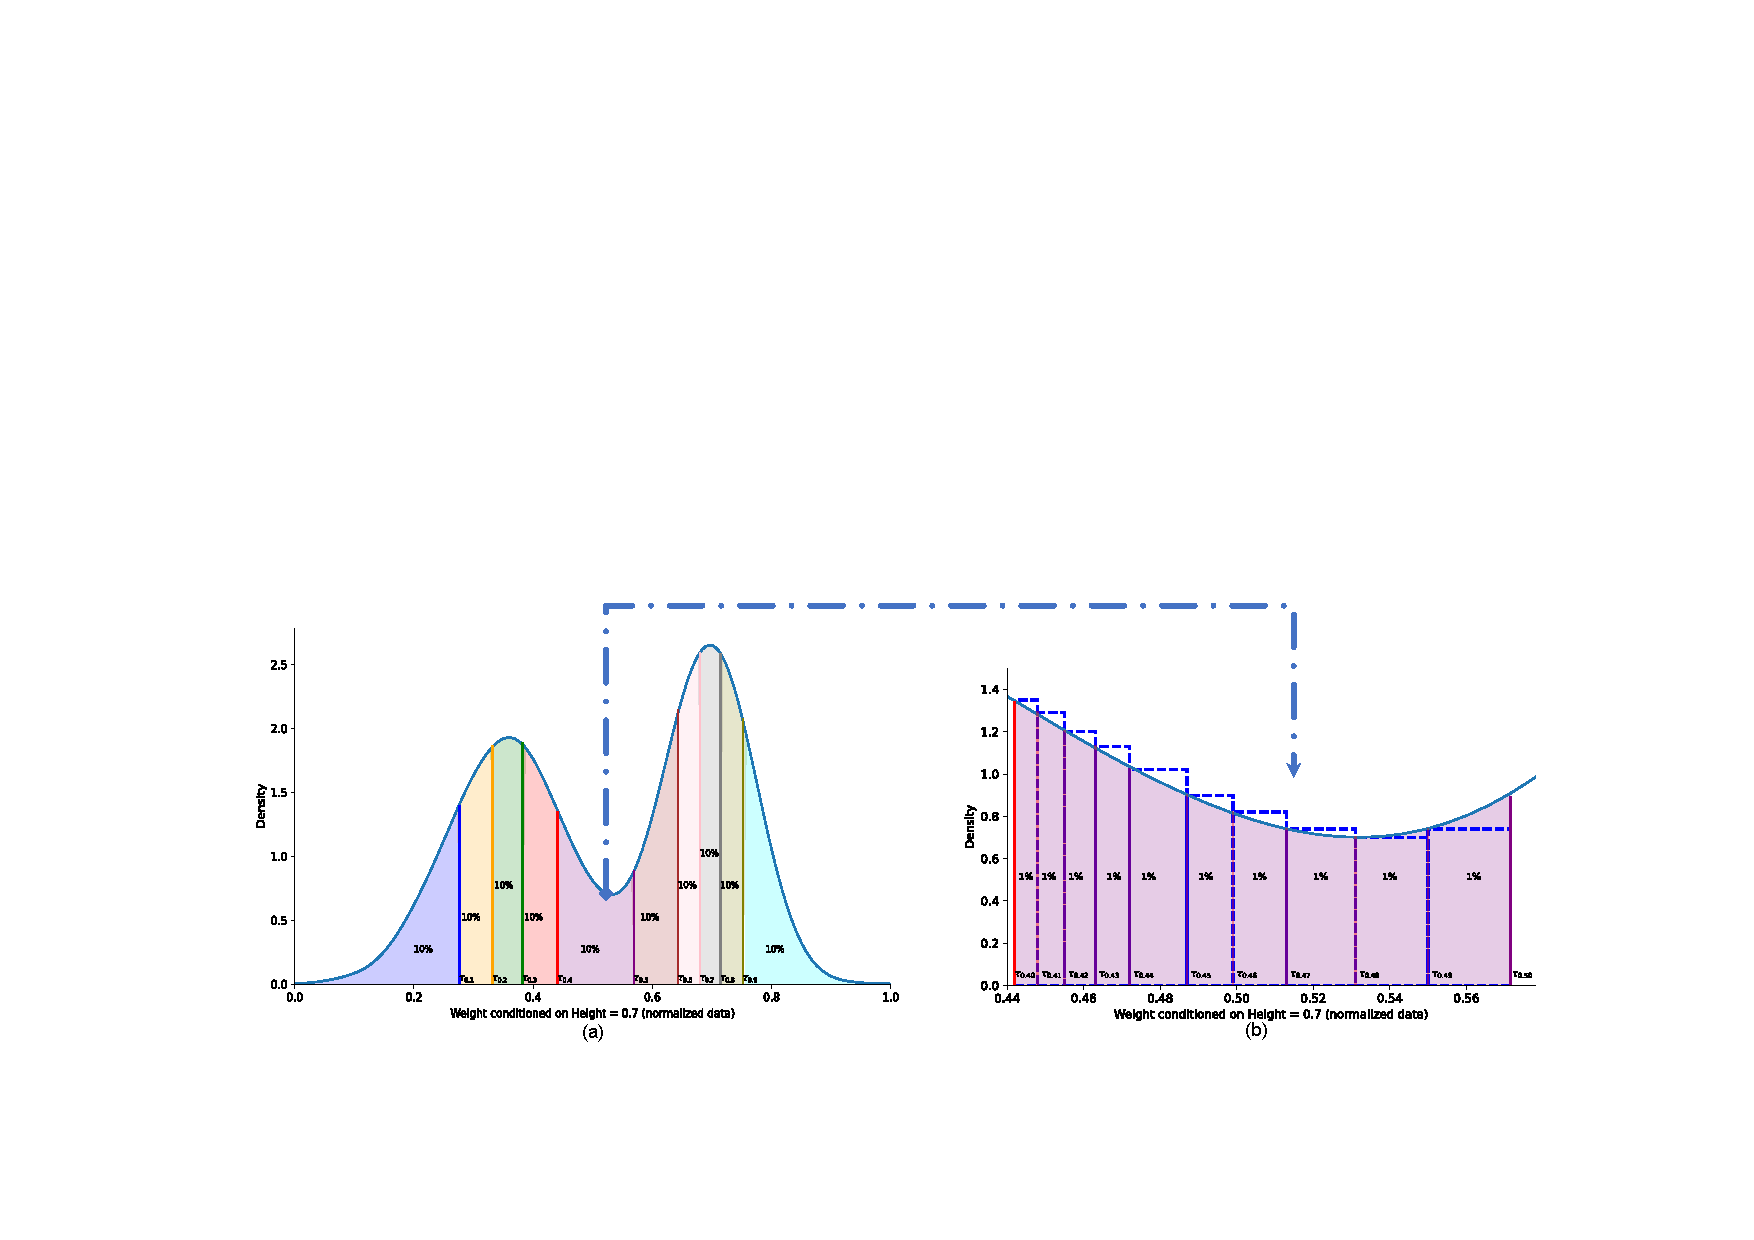
\includegraphics[width=12cm]{images/Pic_quantile_example.pdf}
	\caption{(a) Lượng phân vị có điều kiện ước tính $\{Q_{0.1}, Q_{0.2}, \ldots ,Q_{0.9}\}$ cho một đặc trưng hành vi dựa trên các đặc điểm ngữ cảnh. (b) Phóng to khu vực giữa $Q_{0.40}$ và $Q_{0.50}$, chúng tôi thấy rằng các phân vị có nhiều khả năng đủ chi tiết hơn các phân vị trong (a).}\label{fig:quantile}
\end{figure}

Đây là lúc các khu rừng hồi quy phân vị phát huy tác dụng: được cung cấp đủ dữ liệu huấn luyện, chúng tìm hiểu chính xác hàm phân phối tích lũy có điều kiện, hàm này có thể được truy vấn ở dạng nghịch đảo, tức là thông qua các phân vị có điều kiện. Khi truy vấn một khu rừng hồi quy phân vị, điều này có thể được thực hiện ở các mức độ chi tiết khác nhau. Ví dụ: Hình~\ref{fig:quantile}(a) cho thấy rằng lượng phân vị có điều kiện $\{Q_{0.1}, Q_{0.2}, \ldots ,Q_{0.9}\}$ rất có thể không đủ để mô tả chính xác phân bố có điều kiện vì chúng làm trơn quá mức phân bố cơ bản và do đó không thể nắm bắt chính xác các sắc thái, trong khi Hình~\ref{fig:quantile}(b) cho thấy \emph{percentiles} có điều kiện, tức là, $\{Q_{0.01}, Q_{0.02}, \ldots ,Q_{0.99}\}$ có nhiều khả năng cung cấp đầy đủ chi tiết hơn.

Chúng tôi sử dụng phân vị có điều kiện cho điểm bất thường vì chúng cung cấp mức độ chi tiết cao trong khi không yêu cầu lượng dữ liệu quá lớn để ước tính chính xác.
Là một lợi ích bổ sung, sự khác biệt giữa mỗi phần trăm liên tiếp luôn được đánh giá bằng sự kết hợp có trọng số của số lượng điểm dữ liệu huấn luyện có thể so sánh được, tức là với chi phí làm mịn, chúng tôi không phải chịu ước tính mật độ cục bộ cực kỳ kém ở các khu vực có mật độ thấp.

Để chính thức phát triển điểm bất thường, trước tiên chúng tôi xác định $\tau_i$ là phân vị $i$th, tức là $\tau_i = Q_{i/100}, \forall i \in [0,100]$. Đối với bất kỳ \emph{percentile interval} nào, tức là một khoảng $[\tau_i, \tau_{i+1}]$ được xác định bởi hai phân vị liên tiếp $i$ và $i+1$, theo định nghĩa, chúng ta có định nghĩa rằng nó bao trùm chính xác xác suất $0.01$ (xem Hình~\ref{fig:quantile}(b)). Chúng tôi có thể ước tính mật độ cục bộ của một khoảng phần trăm và sử dụng mật độ đó cho điểm bất thường của mình, nhưng chúng tôi hướng tới điểm số trở nên lớn hơn khi một điểm dữ liệu được coi là bất thường hơn.Để đạt được mục đích này, chúng tôi xác định \emph{độ rộng khoảng phần trăm} $w_i$ là sự khác biệt giữa hai phần trăm liên tiếp $i$ và $i+1$, tức là $\tau_{i+1} - \tau_i$. Như vậy, độ rộng khoảng có thể được coi là 'mật độ nghịch đảo', nghĩa là chiều rộng sẽ tăng khi mật độ cục bộ giảm. Ví dụ, trong Hình~\ref{fig:quantile}(b), chúng ta có $\tau_{46} = 0.5$ và $\tau_{47} = 0.513$, mang lại $w_{46} = 0.013$. Các điểm dữ liệu nằm trong các khoảng phân vị có độ rộng tương đối lớn có nhiều khả năng là các điểm bất thường theo ngữ cảnh hơn, vì chúng nằm trong các khu vực có mật độ thấp của phân bố có điều kiện.

Do đó, ý tưởng cơ bản là xác định điểm bất thường cho đối tượng $\mathbf{x}$ và đặc trưng hành vi $\mathbf{b}^{q}$ là $w(\mathbf{x}\rvert\mathbf{b}^{q})$, tức là độ rộng của khoảng phân vị (được dự đoán bằng QRF) trong đó giá trị hành vi của điểm dữ liệu rơi vào. Tuy nhiên, chúng ta cần xem xét một trường hợp đặc biệt: giá trị đặc trưng hành vi thực tế $b^{q}$ có thể nhỏ hơn phân vị có điều kiện ước tính nhỏ nhất, tức là $\tau_{0}^{q}$ hoặc lớn hơn phân vị có điều kiện ước tính lớn nhất, tức là $\tau_{100}^{q}$. Nghĩa là, giá trị thực tế có thể không rơi vào bất kỳ khoảng phân vị có điều kiện ước tính nào. Để giải quyết vấn đề này, chúng tôi ngoại suy ngoài $\tau_{0}^{q}$ và $\tau_{100}^{q}$, dẫn đến điểm bất thường trung gian

\begin{equation}
\centering
is(\mathbf{x}\rvert\mathbf{b}^{q})=\left\{
\begin{aligned}\left(1+\frac{\tau_{0}^{q}-b^{q}}{\tau_{75}^{q}-\tau_{25}^{q}}\right)\mathrm{max}(w(\mathbf{x}\rvert\mathbf{b}^{q}))&, \text{ if } b^{q} < \tau_{0}^{q} ; \\
\left(1+\frac{b^{q}-\tau_{100}^{q}}{\tau_{75}^{q}-\tau_{25}^{q}}\right)\mathrm{max}(w(\mathbf{x}\rvert\mathbf{b}^{q}))&, \text{ if }  b^{q} > \tau_{100}^{q}, \\
w(\mathbf{x}\rvert\mathbf{b}^{q})&, \text{ otherwise},\\
\end{aligned}
\right.
\label{eq4}
\end{equation}
trong đó $\mathrm{max}(w(\mathbf{x}\rvert\mathbf{b}^{q}))$ biểu thị độ rộng khoảng tối đa của tất cả các khoảng phân vị có điều kiện cho đặc trưng hành vi $\textbf{b}^{q}$.

Thật không may, việc sử dụng trực tiếp Equation~(\ref{eq4}) làm điểm bất thường một phần sẽ khiến cách tiếp cận của chúng ta dễ dẫn đến cái gọi là \textbf{hiệu ứng chính tả}: việc tính tổng điểm từng phần như vậy cho một điểm dữ liệu mà \emph{mạnh mẽ} sai lệch chỉ trong một đặc trưng hành vi \emph{vài} sẽ dẫn đến điểm bất thường lớn hơn dữ liệu dị thường điểm sai lệch vừa phải trong các đặc trưng hành vi của \emph{nhiều}. Kết quả là, những điểm dữ liệu có ít độ lệch lớn sẽ “quyết định” điểm cao nhất; điều này là không mong muốn.

Để tránh hiệu ứng độc tài, chúng tôi cắt bớt điểm bất thường từng phần đến mức tối đa được xác định trước và đi đến điểm bất thường từng phần cuối cùng như

\begin{equation}
\centering
s(\mathbf{x}\rvert\mathbf{b}^{q})=\left\{
\begin{aligned} \frac{\eta}{100} &, \text{ if } is(\mathbf{x}\rvert\mathbf{b}^{q}) > \frac{\eta}{100}; \\
is(\mathbf{x}\rvert\mathbf{b}^{q})&, \text{ otherwise}, \\
\end{aligned}
\right.
\label{eq6}
\end{equation}trong đó $\eta$ là siêu tham số. Cơ sở lý luận cho $\eta$ như sau: nếu phân bố có điều kiện được phân bố đồng đều và đặc trưng hành vi có phạm vi $[0,1]$ thì chiều rộng dự kiến ​​của bất kỳ chiều rộng khoảng phân vị nào là $0.01$ và $\eta$ có thể được hiểu là số lượng tối đa của \emph{độ rộng khoảng phân vị dự kiến}. Trong các thử nghiệm, chúng tôi sử dụng $\eta = 10$ vì hiệu suất thực nghiệm mạnh mẽ của nó (cũng được thể hiện trong nghiên cứu cắt bỏ ở Phụ lục ~ \ref{Appendix:Ablation}).

Bằng cách chia tỷ lệ các đặc trưng hành vi thành $[0,1]$ trước khi phát hiện sự bất thường, ví dụ: sử dụng chuẩn hóa tối thiểu-tối đa, phần trăm có điều kiện ước tính cũng phải nằm trong khoảng này và do đó, độ rộng khoảng thu được cho các đặc trưng hành vi riêng lẻ sẽ có thể so sánh được. Đổi lại, điều này ngụ ý rằng chúng có thể được tính tổng để có được điểm bất thường cuối cùng cho một điểm dữ liệu (Thuật toán~\ref{algo:QCAD}, Dòng 9).

\subsection{Giải thích sự bất thường bằng biểu đồ beanplot bất thường}
\label{qcad:ae}

Trong giai đoạn thứ ba, chúng tôi đưa ra lời giải thích cho những điểm bất thường được báo cáo. Từ định nghĩa về điểm bất thường của chúng tôi, rõ ràng đó là \textit{có thể phân bổ}: điểm tổng thể có thể được phân tách thành một phần điểm cho các đặc trưng hành vi riêng lẻ.

Đối với mỗi điểm bất thường được xác định $\mathbf{a}$, chúng tôi báo cáo các lân cận theo ngữ cảnh của nó là $R(\mathbf{a})$ và điểm bất thường cuối cùng được tính toán trên Dòng~9 của Thuật toán~\ref{algo:QCAD}. Hơn nữa, chúng tôi báo cáo điểm bất thường một phần tương ứng với các đặc trưng hành vi, tức là chúng tôi báo cáo $s(\mathbf{x}\rvert\mathbf{b}^{q})$ cho tất cả $q$, được xếp hạng từ cao nhất đến thấp nhất để cho biết đặc trưng hành vi nào có sự bất thường sai lệch nhiều nhất.

\begin{figure}[tb]
	\centering
	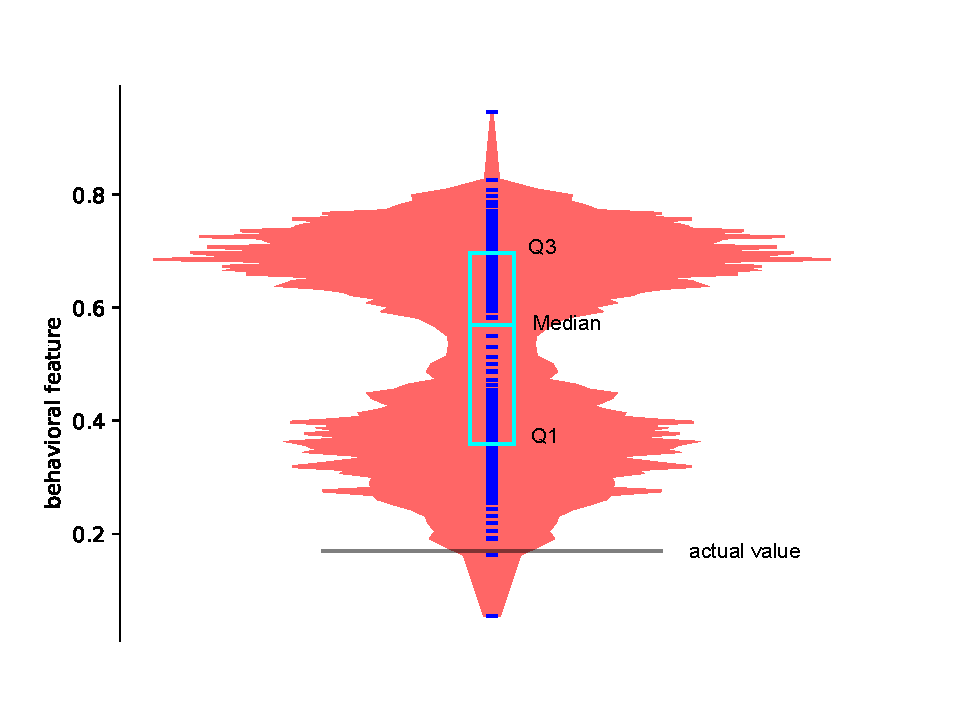
\includegraphics[width=9cm]{images/Pic_beanplot.pdf}
	\caption{Biểu đồ bất thường cung cấp cái nhìn sâu sắc về những gì rừng hồi quy phân vị đã học được đối với một điểm dữ liệu và đặc trưng hành vi cụ thể cũng như lý do tại sao điểm dữ liệu đó (không) được coi là điểm bất thường. Các đường ngắn màu xanh lam biểu thị phần trăm có điều kiện $\tau_0,\tau_1,\ldots,\tau_{100}$ mà QRF đã học được (từ trên xuống dưới), đối với điểm dữ liệu và đặc trưng hành vi nhất định. Như trong biểu đồ hình hộp, hộp (màu lục lam) biểu thị tứ phân vị thứ nhất ($\tau_{25}$), trung vị ($\tau_{50}$) và tứ phân vị thứ ba ($\tau_{75}$). Vùng màu đỏ rộng hơn biểu thị mật độ xác suất được ước tính dựa trên phân vị có điều kiện. Cuối cùng, đường màu đen biểu thị giá trị thực tế mà điểm dữ liệu có.}\label{fig:beanplot}
\end{figure}

Vì trực quan hóa thường giúp nhanh chóng cung cấp thông tin chi tiết có giá trị nên chúng tôi đề xuất \emph{beanplot bất thường}, một biến thể của Beanplot của \cite{kampstra2008beanplot}. Hình~\ref{fig:beanplot} hiển thị một ví dụ, mô tả trực quan các phần trăm có điều kiện đã học, độ rộng khoảng của chúng và mật độ xác suất có thể được ước tính từ những phần trăm đó, tất cả đều dành cho một điểm dữ liệu cụ thể và đặc trưng hành vi. (Hãy nhớ rằng rừng hồi quy phân vị được học trên nhóm tham chiếu của một điểm dữ liệu, do đó biểu đồ beanplot bất thường cho mỗi điểm dữ liệu có thể khác nhau.)Bằng cách đưa giá trị thực tế của điểm dữ liệu vào biểu đồ Beanplot (dưới dạng một đường màu đen nằm ngang), nhà phân tích có thể dễ dàng thấy giá trị đặc trưng hành vi của nó được định vị như thế nào so với giá trị của nhóm tham chiếu và tại sao cũng như ở mức độ nào nó đóng góp vào sự bất thường của nó.
